\documentclass[a4paper]{article}
\usepackage {changepage}
\usepackage{fancyhdr}
\usepackage {fontspec}
\usepackage {paralist}
\usepackage {multicap}
\pagestyle{fancy}
\setromanfont{Lantinghei SC Extralight}
\setmonofont{Courier New}
\XeTeXlinebreaklocale ``zh''
\XeTeXlinebreakskip = 0pt plus 1pt
\textheight = 650pt
\begin{document}
\title{实验报告 Lab 6}
\author{姓名:王钦\quad 学号:13349112}
\date{}
\maketitle

\section*{ Part I: Understanding minisniff}
\hangindent=4em \hangafter=-200{
	\begin{enumerate}
		\item use pcap libaray.I can find more information on http://www.tcpdump.org/
		\item Advantage
		\begin{itemize}
			\item easy to use
			\item compatible with other programs
			\item compatible with operat system both windows and linux
			\item capture all incoming and outgoing packets
		\end{itemize}
		\item Disadvantage
		\begin{itemize}
			\item writen on C language,not have python java etc. other language version.
			\item if dont have computer basic knowledge. it's difficult to learn.
		\end{itemize}
		\item Yes,I have searched on github and find some open source repositories like this one \verb|https://github.com/AnwarMohamed/Packetyzer|
		\item Explain functions(use man command on linux)
		  \begin{itemize}
			  \item  \verb|pcap_lookupdev| - find the default device on which to capture
			  \item \verb|pcap_open_live| - open a device for capturing
			  \item \verb|pcap_lookupnet| - find the IPv4 network number and netmask for a device
			  \item \verb|pcap_compile| - compile a filter expression
			  \item \verb|pcap_setfilter| - set the filter
			  \item \verb|pcap_next| - read the next packet from a \verb|pcap_t|
			  \item \verb|pcap_loop| - process packets from a live capture or savefile
			  \item \verb|pcap_dispatch| - process packets from a live capture or savefile
		  \end{itemize}
		\item on transport layer,because I can find some fields which only show in transport layer such as protocol and total length.
	\end{enumerate}
}
\section*{ Part II: Extending minisniff}
\hangindent=4em \hangafter=-200{
	\begin{enumerate}
	\item I modify some code in \verb|capture.c| file see below 
	  \begin{center} 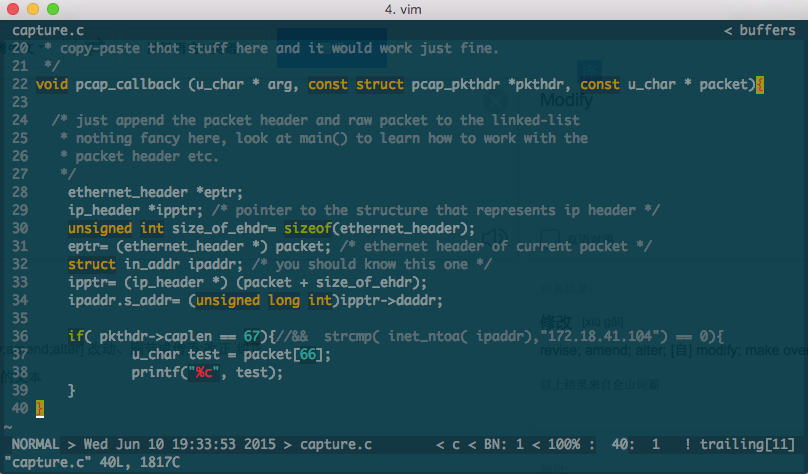
\includegraphics[scale=0.5]{Illustrations/2.png} \mfcaption{minisniff}\end{center}
	\item screetshots see below ,all code is in minisniff folder.User is tsunami,password is 1. server is 172.18.187.113 linux which is my computer in Laboratory.I use macbook as clinet sent telnet to server.
	  \begin{center} 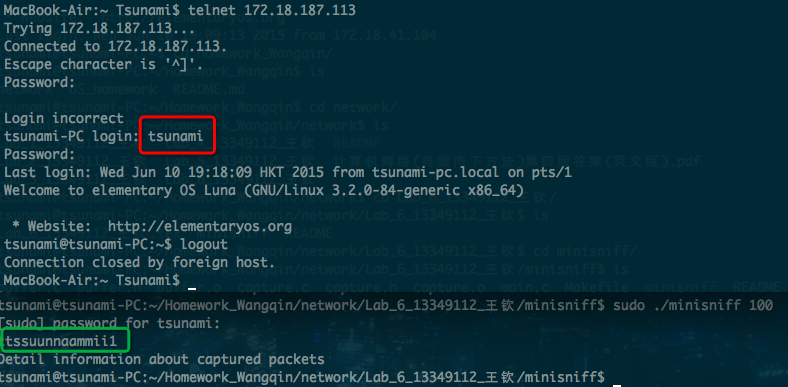
\includegraphics[scale=0.5]{Illustrations/1.png} \mfcaption{minisniff}\end{center}
	\end{enumerate}
\end{document}




